\documentclass[margin,line,a4paper]{resume}

\usepackage[utf8]{inputenc} %utf8
\usepackage[english,danish]{babel}
\usepackage[T1]{fontenc}
\usepackage{graphicx,wrapfig}
\usepackage{url}
\usepackage[colorlinks=true, a4paper=true, pdfstartview=FitV,
linkcolor=blue, citecolor=blue, urlcolor=blue]{hyperref}
\pdfcompresslevel=9


\begin{document}
{\sc \Large Curriculum Vitae -- Adam Jacobs}
\begin{resume}
    \vspace{0.01cm}
    \begin{wrapfigure}{R}{0.25\textwidth}
        \vspace{-1cm}
       \begin{center}
       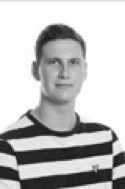
\includegraphics[width=0.15\textwidth]{adamjacobs}
       \end{center}
        \vspace{-1cm}
    \end{wrapfigure}
    
    \section{\mysidestyle Information}%\vspace{2mm}
    Adam Feldstein Jacobs \\
    tel: +46704799492 \\
    email: jacobs\_feld@hotmail.com
    \href{} \\

\section{\mysidestyle Profile}\vspace{1mm}
Using optimism and curiosity to lead technological innovation. I use my experience in leading digitalization projects and hands-on knowledge of software engineering in production as a toolbox. Realizing amazing tech as viable business to customers, and learning new tech makes my clock tick. My core philosophy are (1) performance is achieved via effort - if you don't know enough then learn! (2) Don't be the smartest person in the room! (3) Have the courage to stand out and spread courage to others since it is needed for tough decisions and being innovative! 

\section{\mysidestyle Education}\vspace{1mm}
    \begin{description}
        \item[KTH] Computer Science and MSc Machine Learning (grad. 2022)
         \item[Leadership] course for children summer camps
    \end{description} 

\section{\mysidestyle Projects and Volunteering}\vspace{1mm}
\begin{description}
   \item[Personal Projects] https://github.com/worldyn. Everything from machine learning to system programming to web applications
    \item[Bachelor Thesis using GANs] Effects of Transfer Learning on Data Augmentation with Generative Adversarial Networks. Over 300 views on kth.diva-portal.org!
    \item[Chairman] Nomination Committee (THS)
    \item[Jury Member] Business Model Awards 2020 
    \item[Board Member] Tekniska Högskolans Studentkår (THS) (july 2019-2020)
    \item[System Developer] THS Armada Career Fair 2017. Backend and DevOps
    \item[Team Leader] for 10 people at company Greenlytics, soft. engineer. course 2017. Data Mining and filtering for their ML algos.
    \item[App Developer] Rudbeck Gymnasium (Awarded tech project) 2016

\end{description}  
  
\section{\mysidestyle Work Exp.}\vspace{1mm}
\begin{description}
   \item[Junior Project Manager] Urban ICT Arena, coordinating IOT projects in public sector (summer 2020)
    \item[Intrapreneur] Ericsson ONE incubator, developed business concept with startup within smart grids (summer 2019)
    \item[Student Representative] Inspirational lectures and tour at KTH for pupils that won a programming contest.
    \item[Software Engineer] Ericsson Internship, applying the magic of SR-IOV in cloud orchestration systems (summer 2018)
    \item[Freelancing] Developed and sold task management system to schools (summer 2017)
    \item[Developer] educational resources app, Rudbeck Gymnasium (summer 2016)
    \item[Freelancing] Web developer for UF-companies (2016)
\end{description}

\section{\mysidestyle References and Links}
\begin{description}
    \item[Linkedin] https://www.linkedin.com/feed/
    \item[Written] references handed in per request.
    \item[GitHub] https://github.com/worldyn
\end{description}

\end{resume}
\end{document} 